%% evenend-typography-ja.tex：evenendパッケージのタイポグラフィ編（マクロタイポグラフィの観点から，
%% 紙面の構成として何をどう揃えるか）
%% LuaLaTeXで2回組む．見本（evenend-sample*.pdf）を先に組んでおくこと
\documentclass[paper=a4,fontsize=10pt]{jlreq}
\usepackage{graphicx}
\usepackage{array}
\usepackage{tikz}
\usepackage{hyperref}
\hypersetup{hidelinks,pdftitle={evenendパッケージの組版},pdfauthor={木枝祐介}}

%% ロゴ（クラスやパッケージが定義していなければ定義する）
\providecommand\LuaTeX{Lua\TeX}
\providecommand\LuaLaTeX{Lua\LaTeX}
\newcommand\cs[1]{\texttt{\textbackslash #1}}
%% 制御綴の「\」と和文の間にも和欧文間のアキを入れる（LuaTeX-jaの既定では入らない）
\ltjsetparameter{alxspmode={`\\,allow}}
\newcommand\opt[1]{\texttt{#1}}
\newcommand\pkg[1]{\textsf{#1}}
%% 強調：和文はゴシック体，欧文はイタリック体
\newcommand\kyocho[1]{{\gtfamily\itshape #1}}
%% オプションの見本（evenend-sample-options.pdf）のページ：見本を組むと書き出される
%% evenend-sample-options.pg から読む
\makeatletter\InputIfFileExists{evenend-sample-options.pg}{}{}\makeatother
\newcommand\optpage[2][.4\linewidth]{%
  \fbox{\includegraphics[page=\csname evs@#2\endcsname,width=#1]{evenend-sample-options.pdf}}}
%% 2つの見本を並べ，それぞれの下に説明を付ける：\optpair{見本A}{説明A}{見本B}{説明B}
\newcommand\optpair[5][.4\linewidth]{%
  \begin{tabular}{@{}c@{\hspace{2\zw}}c@{}}
    \optpage[#1]{#2} & \optpage[#1]{#4} \\[.3\baselineskip]
    \small #3 & \small #5
  \end{tabular}}
%% ほかの見本の2ページを並べる：\samplepair{ファイル}{ページA}{説明A}{ページB}{説明B}
\newcommand\samplepair[5]{%
  \begin{tabular}{@{}c@{\hspace{2\zw}}c@{}}
    \fbox{\includegraphics[page=#2,width=.4\linewidth]{#1}} &
    \fbox{\includegraphics[page=#4,width=.4\linewidth]{#1}} \\[.3\baselineskip]
    \small #3 & \small #5
  \end{tabular}}
%% 模式図：x=1mm，y=-.25mm（縦は1ptを0.25mmとし，下向き）で描く
%% \tycol[高さ]{x}{y}：段の地，\tylines{x}{1行目のベースライン}{行数}：本文の行，
%% \tybox{x}{y}{高さ}：図表
\newcommand\tycol[3][178]{\fill[black!8] (#2,#3) rectangle ++(20,#1);}
\newcommand\tylines[3]{\foreach \tyi in {1,...,#3}
  {\fill[black!22] (#1,{#2+(\tyi-1)*12-7}) rectangle ++(20,7);}}
%% 表：前後を半行空ける
\newenvironment{hyou}{\par\addvspace{.5\baselineskip}\begin{center}\small}
  {\end{center}\par\addvspace{.5\baselineskip}}
\newcommand\tybox[3]{\fill[black!50] (#1,#2) rectangle ++(20,#3);}

\title{\pkg{evenend}パッケージの組版\\[.5\baselineskip]
  \large マクロタイポグラフィの観点から}
\author{木枝祐介}
\date{v20261124.2}

\begin{document}
\maketitle

この文書では，evenendパッケージが組む紙面を，マクロタイポグラフィの観点から述べる．
紙面の構成として何を揃え，何を揃えないか，揃えきれないときに何を優先するか，その判断を
示す．\TeX{}の仕組みには立ち入らない．使い方はマニュアル（\texttt{evenend-ja.pdf}），
手順とその性質の証明は定式化の文書（\texttt{evenend-theory-ja.pdf}）にある．

見本は，どれもA6判，8ptの\pkg{jlreq}で組み，同じ大きさで示す．横組だけを扱う
（evenendは縦組に対応していない）．「日本語組版処理の要件」（W3C，2020年8月11日版．
以下，要件）の記述を引くときは，節の番号を添える．

\section{マクロタイポグラフィとevenend}

\subsection{この文書の範囲}

タイポグラフィは，扱う大きさで2つに分けて考えられる．
\begin{itemize}
  \item マクロタイポグラフィ：紙面の全体の構成を扱う．判型と版面，段の数と幅，余白，
    見出し・図表・注といった要素の配置，要素の間のアキ，それらの整列と釣り合い．
  \item ミクロタイポグラフィ：本文の細部を扱う．字，字と字の間，約物の前後のアキ，
    行をどこで分けるか，行頭と行末の処理，行と行の間（行送り）．
\end{itemize}
evenendが手を加えるのは，前者だけである．本文の行は，クラスと\LuaTeX-jaが組んだものを
そのまま使う．行の中の字の並びも，行長も，行送りも変えない．evenendは，組み上がった行と
図表と脚注を，紙面のどこに置くかを決め直す．

行送りには，2つの面がある．行送りの値を決めることは，字の大きさと行長に合わせて
読みやすさを整えることで，ミクロタイポグラフィに属する．一方，日本語の組版では，行送りは
基本版面を決める要素の1つでもあり，決まった行送りは，どのページでも行を置く位置の基準に
なる．evenendは，行送りの値には触れない．扱うのは，その行送りから決まる行の位置を，
紙面の基準として守ることで，こちらはマクロタイポグラフィの側にある．

\subsection{マクロタイポグラフィの観点}

この文書では，evenendの判断を，次の観点に分けて述べる．
\begin{itemize}
  \item 構造：版面を段に分け，行送りの位置を紙面の縦の基準にする（\ref{sec:structure}節）．
  \item 釣り合い：本文がページの途中で終わる段組で，左右の段の高さを揃える
    （\ref{sec:balance}節）．
  \item 整列：段の間で，行の位置と，段の上端・下端を揃える（\ref{sec:align}節）．
  \item 余白：揃えるために生じるアキを，どこにまとめるかを決める（\ref{sec:space}節）．
  \item 配置：脚注と図表を，段と版面のどこに置くかを決める（\ref{sec:place}節）．
  \item 区切り：段数の違う段組を1ページに積み，その間のアキで区切りを示す
    （\ref{sec:switch}節）．
  \item 読む順序：揃えた後も，読み進める道筋が1本に保たれるようにする（\ref{sec:order}節）．
  \item 一貫性：ページによって，同じ要素の位置と大きさが変わらないようにする
    （\ref{sec:consistency}節）．
\end{itemize}

\subsection{用語}

\begin{hyou}
  \begin{tabular}{p{.2\linewidth}p{.7\linewidth}}
    \hline
    用語 & この文書での意味 \\
    \hline
    版面 & 本文を組む領域．柱とノンブルは含まない \\
    段，段間，段間罫 & 版面を左右に分けた1つ1つの領域が段，段と段の間のアキが段間，
      段間に引く罫が段間罫 \\
    段組 & 同じ段数で組んだ，ひと続きの段の並び．evenendでは，1ページにいくつかの段組を
      上から積める（マニュアルでは「ブロック」とも呼ぶ） \\
    行送りの位置 & 版面の1行目から行送りごとに並ぶ，行のベースラインの位置．版面の設計で
      決まる行の位置にあたる \\
    字面，字の枠 & 字面は，字が実際に占める範囲．字の枠は，字の外枠（全角の和字なら
      全角の正方形） \\
    見かけの下端 & 段の最後にあるものの，目に見える下端（\ref{sec:bottom}節） \\
    なりゆき & 行が終わった所で止め，段の行数を調整しない組み方 \\
    段抜き & 図表や見出しが，版面の全幅（すべての段）にわたること \\
    段をまたぐ & 図表が，3段組の2段ぶんのように，いくつかの段にわたること（すべての段では
      ない） \\
    図表 & 図と表．本文の流れから離して置くもの（\LaTeX{}のフロート）を指す \\
    \hline
  \end{tabular}
\end{hyou}

\section{構造：版面，段，行送りの位置}\label{sec:structure}

段組の紙面は，2つの基準でできている．
\begin{itemize}
  \item 横の基準：版面の幅を，段数と段間で分けた段．段の左右の端が，本文と図表の
    左右の位置を決める．
  \item 縦の基準：版面の1行目から行送りごとに並ぶ，行送りの位置．各ページの行は，版面の
    設計で決まる行の位置に置くのが原則である（要件2.5.2）．
\end{itemize}
縦の基準は，本文のために決めた行送りを，紙面の全体に延ばしたものである．
紙面の要素（本文の行，見出し，図表，脚注）は，この2つの基準に沿って置く．横の基準は，
段幅で組むかぎり自然に守られる．崩れやすいのは縦の基準で，高さが行送りの倍数でない
ものが段に入るたびに，その後の行が行送りの位置から外れる．

evenendは，段の高さを決め直すときも，この2つの基準を動かさない．段の幅と段間は
変えず，行送りも変えない．動かすのは，段ごとの行の数と，図表と脚注の置き場所，その
まわりのアキだけである．

\section{釣り合い：段の下端を揃える}\label{sec:balance}

\subsection{なりゆきと，揃えた組み方}

段組の本文がページの途中で終わるとき，組み方は2通りある（図\ref{fig:nariyuki}）．
\begin{itemize}
  \item なりゆき：左の段から順に版面の下端まで詰め，行が終わった所で止める．左の段は
    満杯で，右の段は短いか，空になる．
  \item 揃える：各段の行数を平均にして，段の下端を揃える．
\end{itemize}
なりゆきでは，本文の塊が版面の左に寄り，右下に大きな余白が残る．紙面の重さが片側に
かたよる．横組の段組では，改ページなどの直前のページと最終ページで，各段の行数を揃え，
割り切れないときは最も右の段の末尾を空ける（要件2.3.2，4.1.5）．横組では左右の釣り合いが
目に付くからである．\LaTeX{}の段組はなりゆきで組む．evenendは，これを揃えた組み方に
する．

\begin{figure}[tb]
  \centering
  \optpair{enable-false}{なりゆき}{enable-true}{揃えたもの}
  \caption{本文がページの途中で終わる段組．左はなりゆき（\LaTeX{}の組み方），右は段の下端を
    揃えたもの．揃えると，本文の塊は版面の幅いっぱいの長方形になり，余白は下にまとまる}
  \label{fig:nariyuki}
\end{figure}

揃えると，本文の塊は，版面の幅いっぱいの長方形になる．余白は，その下に1つにまとまる．
段の高さは，本文が入り切る最小の高さにするので，下にまとまる余白は最も大きくなる．
本文の塊と余白の境が1本の水平の線になり，紙面の形がはっきりする．

\subsection{余りの行は最右段で空ける}

行数が段数で割り切れないときは，最右段だけを短くする．2段で31行なら16行と15行，3段で
31行なら11行，10行，10行でなく，11行，11行，9行になる．左から詰めていき，余りを最右段に
寄せるので，最右段のほかの段の下端はすべて揃う．欠けるのは，本文の長方形の右下の角
だけである．短い段が途中にあると，下端の線がでこぼこになり，読む順序もたどりにくい
（\ref{sec:order}節）．

\subsection{揃える場所}

段の下端を揃えるのは，段組の本文がページの途中で終わる所である．
\begin{itemize}
  \item 文書の最終ページ
  \item 改ページの直前のページ（\cs{evenendclearpage}で改ページしたとき）
  \item 1段組に戻る直前のページ（\cs{onecolumn}）
  \item 段数を切り換える所と，段組を改める所（\ref{sec:switch}節）
\end{itemize}
満杯のページは，版面の下端で段が揃っているので，そのままにする．

\section{整列：行の位置と，段の端}\label{sec:align}

段組では，隣り合う段が横に並ぶ．1段組では気にならないずれも，隣の段と見比べられて
目に付く．整列には，横に見比べるもの（行の位置）と，段の端（上端と下端）とがある．

\subsection{段の間で行の位置を揃える}

evenendは，段の下端を揃えるために行間を伸び縮みさせない．本文だけの満杯の段を基準にして，
ほかの段は，図表のまわりのアキで高さを合わせる．行送りは変えないので，揃えた段組でも，
行は段の間で横に揃う．

段の下端を揃えることと，行の位置を揃えることは，両立しないことがある．たとえば，分けられ
ない材料（図表や，長い脚注の付いた行）が段の境に来ると，行を1行ずつ送っても下端が合わ
ない．このときevenendは，行の位置を保ち，下端のほうを譲る（\ref{sec:priority}節）．
行間を広げて下端を合わせると，その段だけ行の濃さが変わり，隣の段と行がずれる．縦の基準
（\ref{sec:structure}節）を崩すより，下を空けるほうを選ぶ．

\subsection{図表の前後の行}

図表の高さが行送りの倍数でなければ，その後に続く行は行送りの位置からずれる．横組で
図表を置くときは，前後のアキを均等にするために行の位置からずらす方法と，行の位置に
合わせる方法とがある（要件2.5.2）．段組では隣の段の行と見比べられるので，evenendは
既定で，行の位置に合わせる（\opt{floatgrid=true}．図\ref{fig:grid}）．
\begin{itemize}
  \item 段の上下に置いた図表は，図表とアキを合わせた高さを行送りの倍数に切り上げ，足した
    分を本文との間のアキに加える．
  \item 本文の途中に置いた図表は，直後の行が行送りの位置に乗るように，足りない分を前後の
    アキに半分ずつ足す．段の先頭に来たときは，後ろにだけ足す．
\end{itemize}
足すアキは1行未満である．\opt{floatgrid=false}では，図表のまわりのアキを伸び縮みさせて
段の高さを合わせるので，図表の後の行は行送りの位置からずれる．

\begin{figure}[tb]
  \centering
  \optpair{floatgrid-true}{行の位置に合わせる（既定）}%
    {floatgrid-false}{アキを伸び縮みさせる}
  \caption{図表の後の行の位置（薄い線は行送りの位置）}
  \label{fig:grid}
\end{figure}

図表そのものを行取りして，高さを行送りの倍数にしておけば（\pkg{gyoudori}など），どの
ページでも行はずれない．evenendが行の位置を合わせるのは，evenendが組み直す段だけである
（マニュアルの「フロートの前後の行の位置」の節）．

\subsection{段の下端：どこを下端とみなすか}\label{sec:bottom}

端を揃えるときに合わせるのは，寸法の上の端ではなく，目に見える端である．段の最後に
あるものによって，目に見える下端は違う．evenendは，次の位置を各段の「見かけの下端」
として，これを揃える．
\begin{hyou}
  \begin{tabular}{p{.3\linewidth}p{.6\linewidth}}
    \hline
    段の最後にあるもの & 見かけの下端 \\
    \hline
    本文の行 & 最終行のベースラインから，本文の行の標準の深さだけ下がった位置．段の間で
      最終行のベースラインが揃う \\
    下に置いた図表 & 図表の下端 \\
    段の下端に置いた脚注 & 脚注の最終行のベースラインを，本文で終わる段の最終行の
      ベースラインに揃える \\
    本文の途中に置いた図表 & 図表の領域が行き着く，次の行の字面の下端
      （行の位置を合わせるとき） \\
    \hline
  \end{tabular}
\end{hyou}

本文で終わる段どうしは，行の下端ではなくベースラインで揃える．最終行にだけ深さの大きい字
（欧文の「g」や「y」，下付きの添字など）があっても，その行の位置は変わらない．脚注は
本文より字が小さいが，これも最終行のベースラインで本文の段に揃える（図\ref{fig:bottom}）．

\begin{figure}[tb]
  \centering
  \begin{tikzpicture}[x=1mm,y=-.25mm]
    \tycol[100]{0}{0}\tycol[100]{24}{0}\tycol[100]{48}{0}
    \tylines{0}{10}{8}
    \tylines{24}{10}{4}\tybox{24}{59}{37}
    \tylines{48}{10}{5}
    \draw[line width=.3pt] (48,74) -- ++(7,0);
    \foreach \i in {0,1} {\fill[black!35] (48,{80+\i*9}) rectangle ++(20,5);}
    \draw[densely dashed,line width=.3pt] (-3,94) -- (71,94);
    \node[anchor=west,font=\footnotesize] at (72,94) {最終行のベースライン};
    \node[font=\footnotesize] at (10,112) {本文};
    \node[font=\footnotesize] at (34,112) {下の図表};
    \node[font=\footnotesize] at (58,112) {脚注};
  \end{tikzpicture}
  \caption{見かけの下端．本文で終わる段と脚注で終わる段は最終行のベースラインを，
    下の図表で終わる段は図表の下端を揃える（図表の下端は，本文の行の標準の深さの位置）}
  \label{fig:bottom}
\end{figure}

\subsection{段の上端と，図表の端}

段の上端は，どの段でも版面（または段組）の上端である．上に置いた図表は段の上端に，下に
置いた図表は段の下端に付ける．段をまたぐ図表は，またがる段のあいだで上端と下端の位置を
揃え，段ごとに上下にずれないようにする（\ref{sec:span}節）．

\subsection{段間罫の端}

段間罫は，段の高さいっぱいに引く．段をまたぐ図表が横切る段間では，図表の上に罫を引かず，
本文のある範囲だけに引く．ここでも，罫の端は目に見える端に合わせる．行の字の枠では
なく，字面に合わせる．
\begin{itemize}
  \item 上端：図表の下の最初の行の，字面の上端．段間の両側の段のうち，高いほうに合わせる．
  \item 下端：図表の上の最後の行の，字面の下端．両側の段のうち，低いほうに合わせる．
\end{itemize}
字の枠に合わせると，罫が行より上下に飛び出して見える．字面は，その行に実際にある字の
輪郭から求める．

\section{余白：アキをどこにまとめるか}\label{sec:space}

段の高さを揃えると，どこかにアキが生じる．マクロタイポグラフィでは，アキは余りではなく，
紙面の要素の1つである．同じ量のアキでも，1か所にまとまっていれば区切りや余白として
読めるが，行間に散っていれば組みのむらに見える．evenendは，アキを行間には入れず，
要素と要素の境にまとめる．入れる場所は次のとおりで，上にあるものほど先に使う．
\begin{hyou}
  \begin{tabular}{p{.3\linewidth}p{.6\linewidth}}
    \hline
    場所 & 入れるアキ \\
    \hline
    図表と本文の間 & 図表の高さの，行送りの倍数に足りない分．図表のある段を基準の段に
      合わせる伸び縮み \\
    下の図表の上 & 本文のアキを伸ばしても図表が届かない分．行は行送りの位置のままにして，
      ここを空ける \\
    脚注の上 & 脚注の高さの，行送りの倍数に足りない分 \\
    段組と段組の間 & ページの残りが行送りの位置で終わるための，1行未満の分 \\
    段の下 & 分けられない材料が入らなかった段の，空いた分 \\
    \hline
  \end{tabular}
\end{hyou}

ページ全体では，余白の出方は次のようになる．
\begin{itemize}
  \item 揃えた段組の下の余白は，版面の幅いっぱいに，1つにまとまる．
  \item 脚注を版面の下端に置く組みでは，この余白は本文の段組と脚注の間に入る．本文と
    脚注という2つの領域を，余白が分ける．
  \item 段組を積んだページでは，段組と段組の間のアキが，区切りとして働く
    （\ref{sec:switch}節）．
\end{itemize}

\section{配置：脚注と図表}\label{sec:place}

\subsection{脚注}

横組の脚注は，版面の下側に置く（要件4.2.1）．段組では，置き方が2通りある
（図\ref{fig:footnote}）．紙面の領域の分け方が違う．
\begin{itemize}
  \item 版面の全幅で組み，版面の下端に置く（\opt{footnote=page}，既定）．版面を，上の
    本文の領域と下の脚注の領域とに，水平に分ける．脚注は段に分かれない．段の高さは，
    版面から脚注の領域を除いた高さで，どの段も同じである．
  \item 段幅で組み，参照する箇所のある段の下端に置く（\opt{footnote=column}）．版面を
    段に分けた，その段ごとに本文と脚注を上下に分ける．脚注のある段は，その分だけ本文が
    少ない．
\end{itemize}

\begin{figure}[tb]
  \centering
  \optpair{footnote-page2}{版面の全幅で版面の下端}{footnote-column2}{段の下端}
  \caption{最終ページの脚注}
  \label{fig:footnote}
\end{figure}

最終ページでは，次のようにする．
\begin{itemize}
  \item 版面の下端に置く脚注は，本文がページの途中で終わっても，版面の下端から動かさ
    ない．揃えた段組と脚注の間が空く．脚注の位置がページによって変わらないことを優先
    する（\ref{sec:consistency}節）．
  \item 段の下端に置く脚注は，脚注を含めて段の下端を揃える．本文を分け直すと，参照する
    箇所が別の段へ移ることがある．脚注は，参照する箇所のある段へ一緒に移す．
  \item なりゆきの組みで段をまたいで分かれていた脚注は，1つにまとめ直す．揃える段組では，
    脚注を段をまたいで分けない．
  \item 脚注の高さは行送りの倍数とは限らない．端数は脚注の上のアキで受け，本文の行の
    位置は動かさない．
\end{itemize}

\subsection{段の中の図表}

段幅の図表は，段の上か下に置くのが基本である．段の端に付ければ，本文の流れを途中で
切らず，図表の端が段の端と揃う．揃える段組では，次のようにする．
\begin{itemize}
  \item 図表の番号の順は変えない．
  \item 図表を置く段は，揃えたときの段の高さが最も小さくなるように選び直す．なりゆきの
    組みで置かれた段より前の段へは動かさない．高さが同じなら，動かす図表の少ない置き方に
    する．
  \item 上の図表は段の上端に，下の図表は段の下端に付ける．
  \item 本文の途中に置いた図表は，その位置から動かさない．図表は分けられないので，前後の
    本文の量によっては段の下端が揃わない．
\end{itemize}
図表を動かすのは，段の高さを小さくするためで，参照する箇所との前後は見ていない．参照より
前に図表が来ては困る文書では，置く位置の指定で調整する．

\subsection{段抜きの図表と，段をまたぐ図表}\label{sec:span}

図表の幅は，段の基準に合わせる．1段ぶん，いくつかの段ぶん，版面の全幅のどれかにすれば，
図表の左右の端が段の端と揃う．

段抜きの図表（版面の全幅）は，版面の上か下に置く．揃えた段組は，その下か上に入る．

3段組の2段ぶんのように，いくつかの段にまたがる図表も置ける（図\ref{fig:span}）．
\begin{itemize}
  \item 幅は，またがる段の幅と，その間の段間を合わせた幅にする．
  \item 位置は，段の上か下．またがる段のあいだで，図表の上端と下端の位置を揃える．
  \item 段の下端に脚注を置く組みで，図表を下に置くときは，脚注を図表の上に置く（既定）．
    脚注を図表の下に置くこともでき（\opt{spanfootnote=bottom}），そのときは，またがる
    段のうち最も高い脚注の上に図表を揃える．どちらでも，図表が段ごとに上下にずれることは
    ない．
\end{itemize}

\begin{figure}[tb]
  \centering
  \samplepair{evenend-sample-span.pdf}{1}{上に置いたもの}{2}{下に置いたもの（最終ページ）}
  \caption{3段組で2段にまたがる図}
  \label{fig:span}
\end{figure}

\subsection{箱の中の段組}

枠で囲んだ箱や図表の中でも，段組を組める（図\ref{fig:box}）．箱は，紙面の中のもう1つの
小さな版面にあたる．箱の幅を段数と段間で分け，箱の中の行送りで組み，各段の下端を揃える．
箱の中の行は，箱の外の行送りの位置とは別に並ぶ（箱の中だけ字の大きさを変えることが
多い）．箱の中の段組は，段をまたいで次のページへは続かない．

\begin{figure}[tb]
  \centering
  \samplepair{evenend-sample-nest.pdf}{1}{枠の中，図の中の段組}{2}{最終ページ}
  \caption{段の中に置いた箱の中の段組}
  \label{fig:box}
\end{figure}

\section{区切り：段数の切り換え}\label{sec:switch}

ページの途中で段数を変えられる（2段から3段へなど）．同じ段数のまま，段組を改めることも
できる．切り換えの前の段組は，最終ページと同じように下端を揃え，その下に次の段組を置く
（図\ref{fig:switch}）．1ページが，水平に積んだいくつかの帯に分かれる．帯ごとに
段の数が違ってよい．

\begin{figure}[tb]
  \centering
  \samplepair{evenend-sample-switch.pdf}{1}{見出しの上アキを段の中にとる（既定）}%
    {2}{段組の全体を下げる}
  \caption{2段，3段，1段，2段と切り換えたページ}
  \label{fig:switch}
\end{figure}

\subsection{段組と段組の間}

段組の区切りは，アキで示す．前の段組の最終行から，次の段組の1行目までを，ベースライン
からベースラインまでで決める（\opt{blockskip}．既定は行送りの2倍，つまり1行アキ）．
前の段組の下端が揃っているので，このアキは版面の幅いっぱいの帯になる．行送りの倍数に
しておけば，段数を変えても，行はページの行送りの位置に乗り続ける．

行送りの位置に乗らない材料（行取りしていない見出しなど）が前の段組にあって，ページの
残りが行送りの位置で終わらなくなるときは，段組の間のアキを1行未満だけ広げて，後の段組を
行送りの位置に戻す．

\subsection{見出しで始まる段組}

行取りした見出しは，上下のアキを含めた領域を占める（要件4.1.6）．切り換えた後の段組が
見出しで始まるとき，見出しの上アキの扱いは2通りある（図\ref{fig:switch}）．
\begin{itemize}
  \item 段の中にとる（\opt{headingskip=column}，既定）：見出しは1段目の中で上アキをとり，
    ほかの段の1行目は段組の上端から始まる．段組の間は，どこでも同じ大きさになる．
  \item 段組の全体を下げる（\opt{headingskip=block}）：段組の全体を，見出しの上アキの
    分だけ下げる．段組の間は，節の区切りの分だけ広くなり，1段組に切り換えたときと同じ
    大きさになる．
\end{itemize}
前者は，段組の区切りと節の区切りを別のものとして扱う．後者は，節の区切りを段組の間の
アキに表す．段組を節の区切りで改めるなら，後者のほうが，区切りのアキが段数によらず同じに
なり，区切りの強さがアキの大きさに対応する．

\subsection{ページの残りが少ないとき}

切り換えた後，ページの残りが少ないと，2，3行だけの段組がページの下端にできる．新しい
段組が始まったことが読み取りにくく，紙面の下端に切れ端が残ったように見える．残りが
決まった高さ（\opt{blockmin}．既定は5行分）より小さければ，そこで改ページし，次の
ページから新しい段数で組む．

\subsection{段間と段間罫}

段間と段間罫の太さは，段組ごとに決められる．段数を増やして行長が短くなる段組では，段間を
狭くする，といった使い方ができる．段幅は，版面の幅から段間を除いて段数で割った幅になる
ので，段間を字の大きさの整数倍にしても，行長が字の大きさの整数倍になるとは限らない．
行長を整数倍にしたいときは，版面の幅と段間をそうなるように決めておく．

\subsection{図表と脚注}

図表は，書いた段組の中で完結させる．段数を変えた後の段組に，前の段組の図表が前の段幅の
まま入ることはない．上の図表は段組の上端に，下の図表は段組の下端に置く（ページの上端，
下端ではない）．

脚注は，版面の下端に置く組みでは，そのページのどの段組の脚注もまとめて版面の下端に置く．
段の下端に置く組みでは，参照する箇所のある段組の，その段の下端に置く．

\section{読む順序}\label{sec:order}

段組の紙面は，段を上から下へ読み，次の段の上端へ移る．段組を積んだページでは，上の
段組を読み終えてから下の段組へ移る．evenendは，揃えた後も，この道筋が1本に保たれる
ようにする．
\begin{itemize}
  \item 本文の順序は変えない．段に分け直すだけである．
  \item 短くするのは最右段だけにする．途中の段が短いと，その段の下の余白が，段組の
    終わりに見える．
  \item 段の下端に置く脚注は，参照する箇所と同じ段に置く．読み手は，参照から段の下へ
    目を移せばよい．
  \item 図表の番号の順は変えない．
  \item 段組を積んだページでは，前の段組の下端を揃えてから，次の段組を始める．上の段組の
    終わりが1本の水平の線になり，そこから下が次の段組であることがわかる．
  \item 柱に章や節の見出しを出すときは，ページの最初と最後の見出しを，この読む順序
    （段組は上から，段は左から，段の中は上から）で決める．段の下端を揃えて本文が別の
    段へ移っても，柱は揃えた後の紙面のとおりになる．
\end{itemize}

\section{一貫性}\label{sec:consistency}

同じ要素は，どのページでも同じ位置に，同じ大きさで現れるのがよい．揃えるページだけが
別の組み方に見えないように，evenendは次のものを変えない．
\begin{itemize}
  \item 行送りと行の位置．揃えたページでも，行は行送りの位置に乗る．
  \item 段幅と段間．1つの段組の中では，ページをまたいでも同じである．
  \item 版面の下端に置く脚注の位置．本文が短いページでも，版面の下端にある．
  \item 段の上端．揃えたページでも，段は版面（または段組）の上端から始まる．
  \item 段組と段組の間のアキ．同じ設定なら，どの切り換えでも同じ大きさになる．
\end{itemize}

\section{優先する順}\label{sec:priority}

すべてを同時に満たせないとき，evenendは次の順に守る．下にあるものほど先に譲る．
\begin{enumerate}
  \item 材料を失わず，順序を変えない．分けられないもの（図表，箱，揃える段組の脚注）は
    分けない．
  \item 段は版面からはみ出させない．
  \item 最右段を，ほかの段より高くしない．
  \item 本文の行を，行送りの位置に置く．
  \item 脚注の最終行のベースラインを，本文の段に揃える．
  \item 段の下端を揃える．
\end{enumerate}
観点で言えば，読む順序と版面の枠を最も上に置き，その次に縦の基準（行の位置），最後に
釣り合い（下端）を置く．

揃えた形がページに入り切らないときは，まず，脚注の高さを行送りの倍数に切り上げるのを
やめ，それでも入らなければ，図表の前後の行を行送りの位置に合わせるのをやめる．それでも
入らなければ，揃えずに，なりゆきの組みのままにして警告を出す．

分けられない材料が段の境に来て，行の位置を保ったままでは下端が合わないときは，その段の
下を空ける．アキを行間に散らして下端を合わせることはしない．

\section{体裁の判断と設定}

\begin{hyou}
  \begin{tabular}{p{.34\linewidth}p{.27\linewidth}p{.27\linewidth}}
    \hline
    判断 & 既定 & 別の選び方 \\
    \hline
    脚注を置く場所 & 版面の全幅で版面の下端（\opt{footnote=page}） &
      段の下端（\opt{footnote=column}） \\
    図表の前後の行 & 行送りの位置に合わせる（\opt{floatgrid=true}） &
      アキを伸び縮みさせる（\opt{floatgrid=false}） \\
    段組と段組の間 & 行送りの2倍，つまり1行アキ（\opt{blockskip}） &
      寸法で指定する \\
    見出しで始まる段組の上アキ & 段の中にとる（\opt{headingskip=column}） &
      段組の全体を下げる（\opt{headingskip=block}） \\
    切り換えた後に組む最小の高さ & 5行分（\opt{blockmin}） &
      寸法で指定する \\
    段をまたぐ下の図表と脚注 & 脚注を図表の上（\opt{spanfootnote=above}） &
      脚注を図表の下（\opt{spanfootnote=bottom}） \\
    文書の最終ページ & 揃える（\opt{enable=true}） & なりゆき（\opt{enable=false}） \\
    1段組に戻る直前のページ & 揃える（\opt{onecolumn=true}） &
      なりゆき（\opt{onecolumn=false}） \\
    \hline
  \end{tabular}
\end{hyou}

\section{扱わないこと}

\begin{itemize}
  \item ミクロタイポグラフィ．行の中の字の並び，字間，約物の前後のアキ，行をどこで
    分けるか，行送りの値は，クラスと\LuaTeX-jaが決めたままにする．
  \item 版面の設計．判型，版面の位置と大きさ，行長，1ページの行数，段数，段間は，文書を
    作る側が決める．evenendは，決められた版面の中で配置を決め直す．
  \item 縦組．縦組の段組では，改ページの直前のページをなりゆきにし，各段の行数を揃えなくて
    よい（要件4.1.5）．evenendは縦組に対応していない．
  \item 段の末尾に来た見出しを次の段へ送ることや，段落の最後の1行だけが次の段へ送られない
    ようにすること．行をどこで段に分けてよいかは，クラスと\LaTeX{}の決まり（分けては
    いけない所の指定）に従い，evenendは判断を加えない．
  \item 段抜きの見出しの前で本文を折り返すこと．段数の切り換え（\ref{sec:switch}節）で，
    1段の段組に見出しを置けば，同じ体裁になる．
  \item 見開きの左右のページの釣り合い．evenendは，1ページの中の段だけを揃える．
  \item 満杯のページ．段の下端は版面の下端で揃っているので，組み直さない（脚注を版面の
    全幅で置く組みでは，脚注の領域を除いた高さの段に組み直す）．
\end{itemize}

\end{document}
